\subsection{Reprojection Error}
As shown in Figure \ref{epi}, $P$ is our feature point which can be seen in two keyframes. $P'_1$ and $P'_2$ are point $P$ captured on two keyframe and $P_1$ and $P_2$ are the intersection points of equalvalent camera plane and the lines ($O'P$ and $O''P$) between camera center ($O'$ and $O''$) and feature point $P$. The reprojection error is the distance between $P_1$ and $P'_1$ (as shown in the green). The reprojection error can be optimized by adjusting the camera pose $R$ and translation $t$, which is discussed above.

\subsection{Epipolar Geometry}
\begin{figure*}
    \centering
    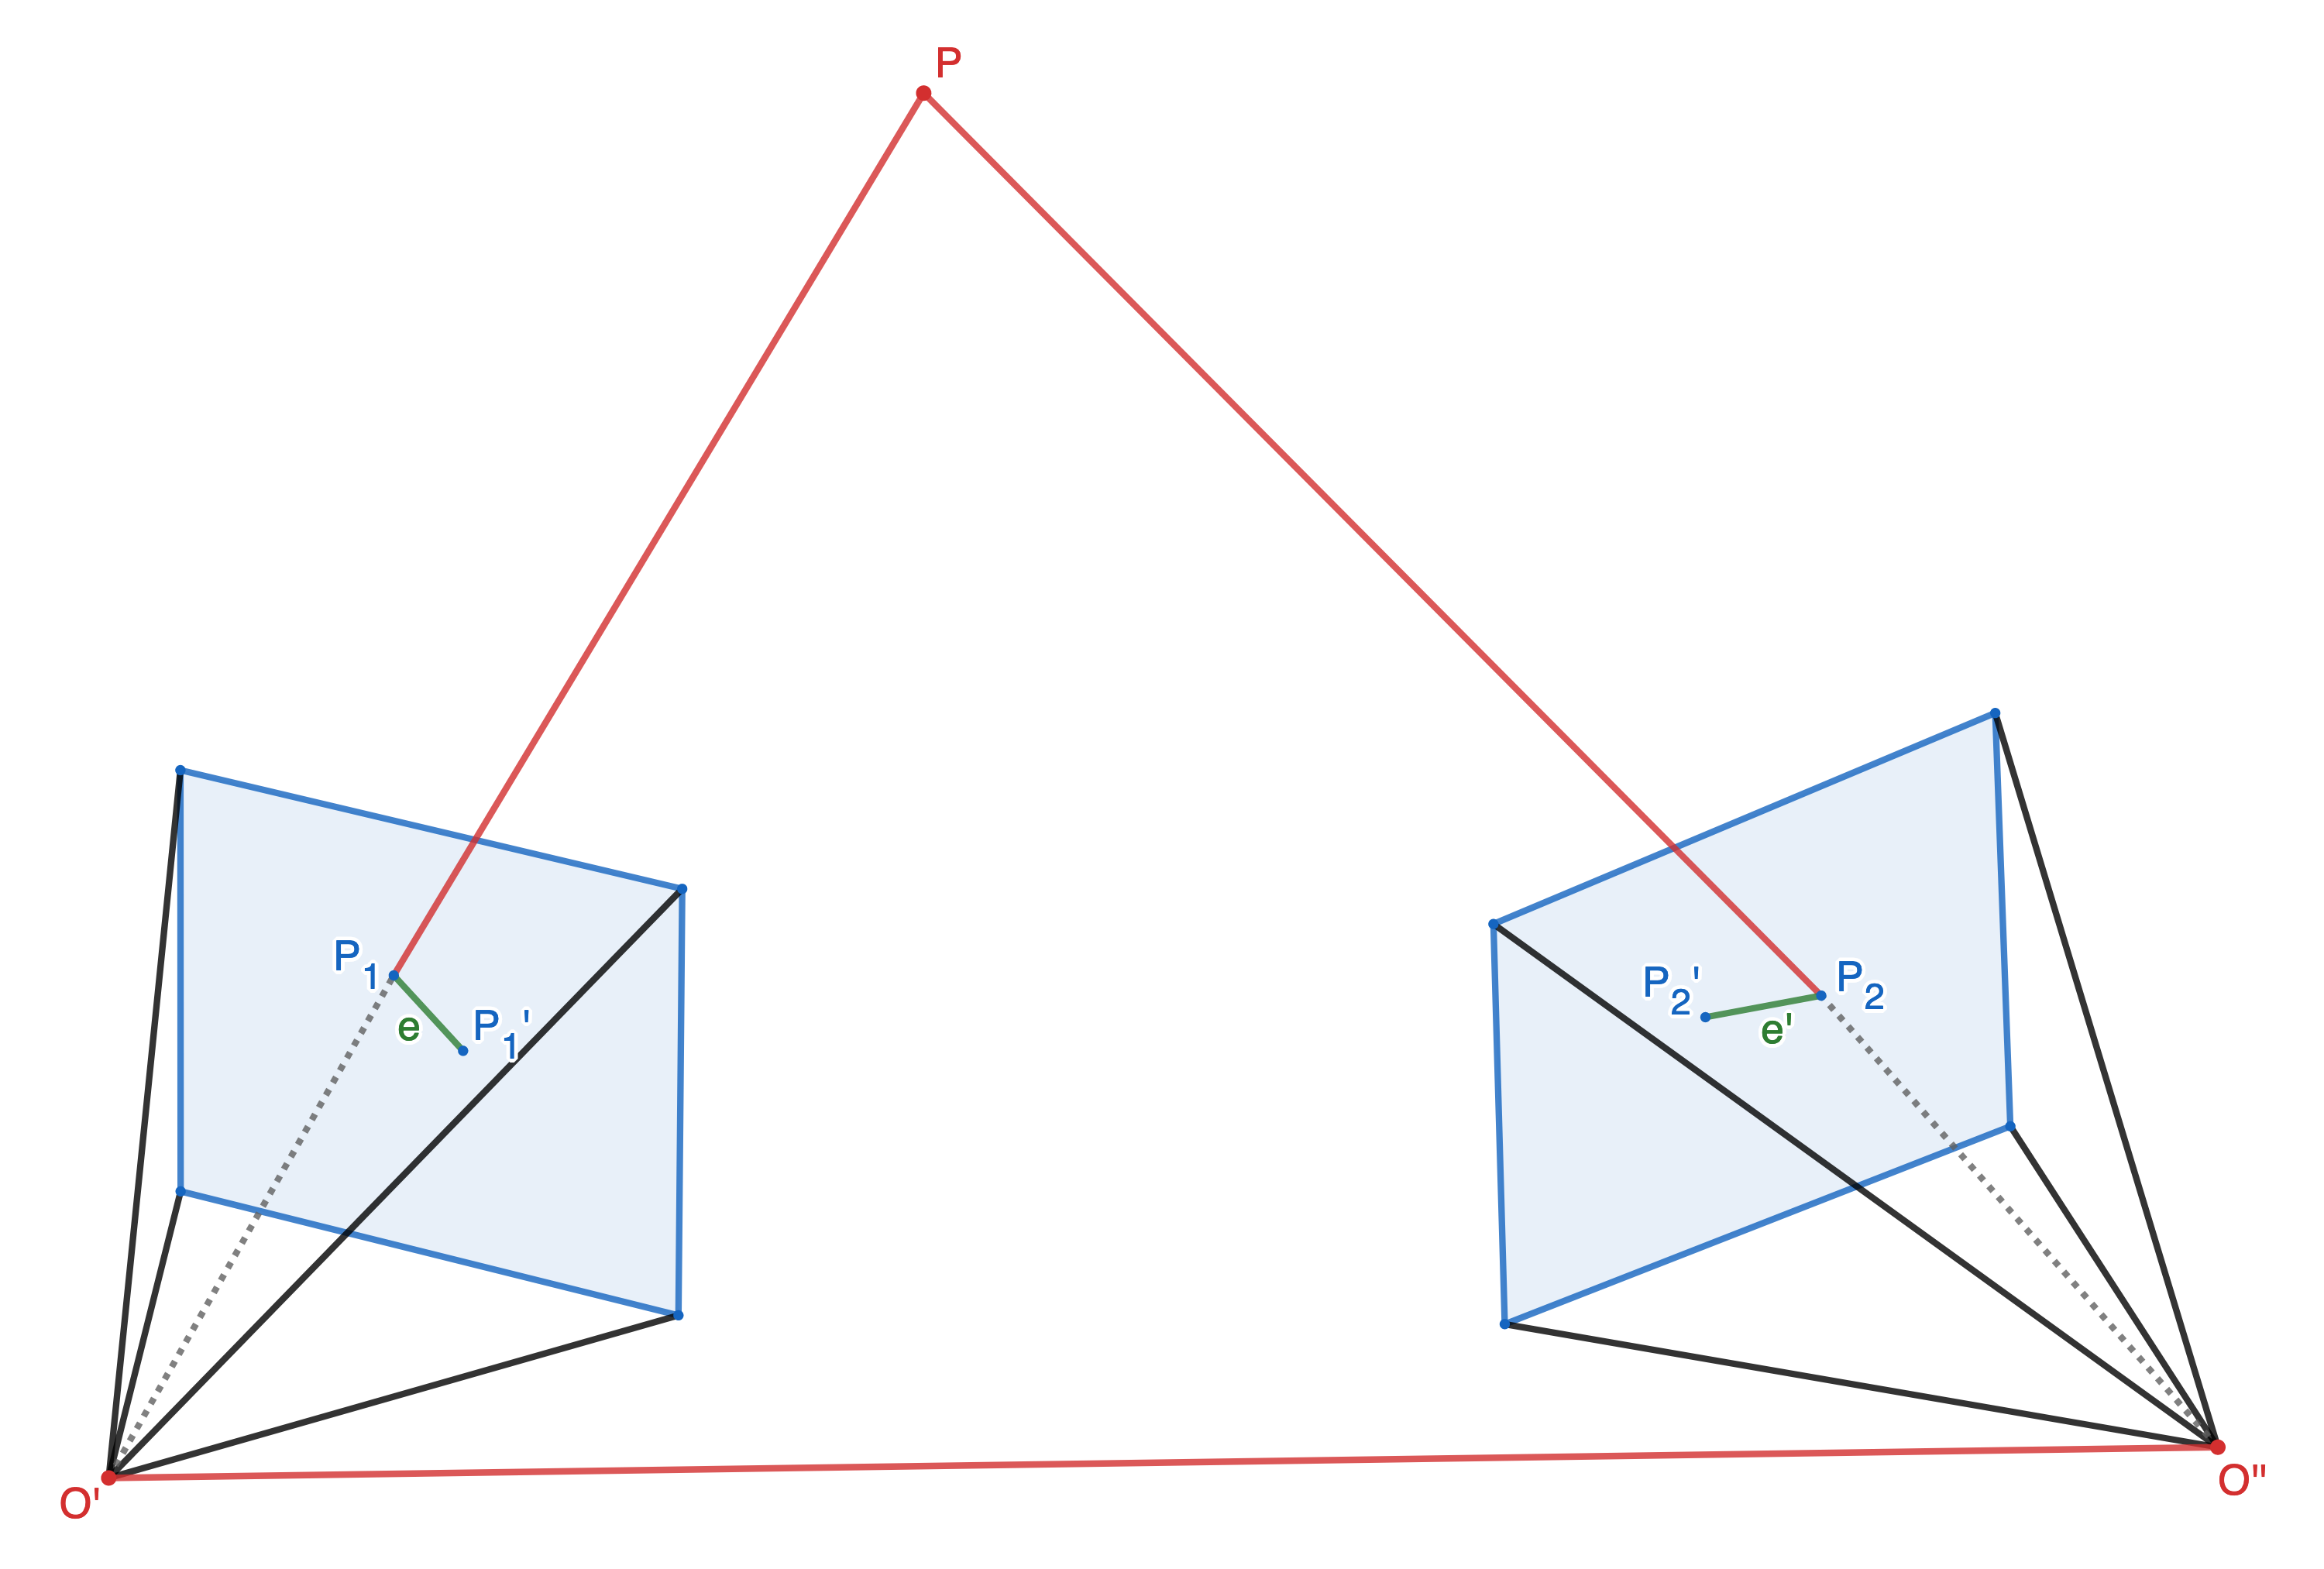
\includegraphics[scale=1.15]{Epipolar.png}
    \caption{Epipolar Geometry and Reprojection Error}
    \label{epi}
\end{figure*}

\begin{align}
    p^T_2K^{-T}t^RK^{-1}p_1 = 0 \\
    E = t^R \\
    F = K^{-T}EK^{-1}
\end{align}\\
where $E$, $F$ are called Essential matrix and Fundamental Matrix.
    Assuming the pixel location of two points are 
\begin{align}
    s_1p_1 &= KP\\
    s_2p_2 &= K (RP + t)
\end{align}\\
where $k$ is the camera's internal matrix, and $R$,$t$ represent the transformation of two frame references.\\
Taking
\begin{align}
     x_1 &= K^{-1}p^{-1} \\ 
     x_2 &= K^{-1}p^{-2}
\end{align}\\
where $x_1$, $x_2$ are the coordinate of two points on equivalent plane where between the film and lens.\\
Get $x_1$, $x_2$ into the above equation, we have:
\begin{equation}
    x_2 = Rx_1 + t \label{1_2}
\end{equation}\\
simplifying the equation by taking the outer proudct of t with both sides of the equation \ref{1_2}, and we get 
\begin{align}
    t^{\wedge}x_2 = t^{\wedge}Rx_1\\
    x^T_2t^{\wedge}x_2 = x^T_2t^{\wedge}Rx_1
\end{align}\\
We can know that the left equation is equal to 0 ,and get:
\begin{equation}
    x^T_2t^{\wedge}RK^{-1}P_1 = 0
\end{equation}
and it also is equal to 
\begin{equation}
    p^T_2K^{-T}t^RK^{-1}p_1 = 0
\end{equation}
\subsection{Euclidean transformation}
The robot can be seen as rigid body when it moving, which means the length and angle keep stable at any frame of reference. Such a transformation called Euclidean transformation. Euclidean transformation include two parts, rotation and translation. Firstly consider rotation. Set the vector $\pmb{\vec{a}}$, the coordinate points are 
$
    \begin{bmatrix} 
        a_1 & a_2 & a_3
    \end{bmatrix} 
$
and 
$
\left[
\begin{matrix} 
    a'_1 & a'_2 & a'_3
\end{matrix} 
\right]^T
$ at two different frame of reference. One of orthogonal basis is 
$
\begin{bmatrix} 
    e_1 & e_2 & e_3
\end{bmatrix} 
$
, after the rotation, it becomes 
$
    \begin{bmatrix} 
        e'_1 & e'_2 & e'_3
    \end{bmatrix} 
$.
$$
   \begin{bmatrix}
        e_1 & e_2 & e_3
   \end{bmatrix} 
   \begin{bmatrix}
    a_1\\
    a_2\\
    a_3
    \end{bmatrix}
    =
    \begin{bmatrix}
    e'_1 & e'_2 & e'_3
    \end{bmatrix}
    \begin{bmatrix}
    a'_1\\
    a'_2\\
    a'_3
    \end{bmatrix}
$$
Then do left multiplication at the same time by 
$
    \left[
    \begin{matrix}
    e_1^T & e_2^T & e_3^T
    \end{matrix}
    \right]^T
$, and the coefficient at left side become identity matrix $\pmb{I}$. We can get the following equation:
$$
    \begin{bmatrix}
        a1\\
        a2\\
        a3
    \end{bmatrix}=
    \begin{bmatrix}
        e^T_1e'_1 & e^T_1e'_2 & e^T_1e'_3\\
        e^T_2e'_1 & e^T_2e'_2 & e^T_2e'_3\\
        e^T_3e'_1 & e^T_3e'_2 & e^T_3e'_3
    \end{bmatrix}
    \begin{bmatrix}
    a'_1\\
    a'_2\\
    a'_3
    \end{bmatrix}
    \triangleq \pmb{Ra}'
$$
The matrix at middle define as rotation matrix $\pmb{R}$, which is composed by two set of orthogonal basis 
$
\begin{bmatrix}
    e_1 & e_2 & e_3 
\end{bmatrix} 
$ and 
$ 
\begin{bmatrix}
    e'_1 & e'_2 & e'_3 
\end{bmatrix}. 
$
The matrix $\pmb{R}$ describes rotation itself, so it also called rotation matrix. Meanwhile, the rotation matrix is an orthogonal matrix with determinant equal to 1. So the set of rotation matrices is defined as follows:
\begin{equation}
    SO(n)=\{\pmb{R} \in \mathbb{R}^{n\times n} | \pmb{R}\pmb{R}^T = \pmb{I}, det(\pmb{R}) = 1\}
\end{equation}
where $SO(n)$ is the meaning of special orthogonal group. In particular, $SO(n)$ is the rotation of three-dimensional space. In the Euclidean transformation, there is a translation in addition to the rotation.
Consider the vector $\pmb{a}$ at world coordinate system, after once rotation (present by \pmb{R}) and once translation $\pmb{t}$, getting $\pmb{a}'$. Then put the rotation and translation together we have the following equation.
\begin{equation}
\pmb{a}'=\pmb{Ra} + \pmb{t}
\end{equation}
The \pmb{t} is defined as translation vector. Compared to rotation, translation is just adding together. By the above equation, we use a rotation matrix $\pmb{R}$ and a translation vector $\pmb{t}$ to completely describe the coordinate transformation relationship of an Euclidean space.

\subsection{Homogeneous coordinates}

At the above, we use a rotation matrix $\pmb{R}$ and a translation vector $\pmb{t}$ to completely describe the coordinate transformation relationship of an Euclidean space.
But there is a problem. When do several times transformation,the equation will become complex and not linear relation. So here introduce the Homogeneous coordinates and transformation matrix rewriting.

\begin{equation}
    \begin{bmatrix} 
        \pmb{a}' \\
        1
    \end{bmatrix}=
    \begin{bmatrix}
        \pmb{R} & \pmb{t}\\
        \pmb{0}^T & 1
    \end{bmatrix}
    \begin{bmatrix}
        \pmb{a}\\
        1
    \end{bmatrix}
    \triangleq
    \pmb{T}\\
    \begin{bmatrix}
        \pmb{a}\\
        1
    \end{bmatrix}
\end{equation}
Thus homogeneous coordinate is adding 1 to the end of a 3-dimensional vector then it become a 4-dimensional vector. As for the 4-dimensional vector, we put the rotation and transformation into one matrix. At the equation, the matrix $\pmb{T}$ defined as transform matrix, and using $\pmb{\tilde{a}}$ to present homogeneous coordinates of $\pmb{a}$.

\subsection{Transformation matrix}

For the transformation matrix, it has special structure: top left corner is rotation matrix, top right corner is translation vector, bottom left corner is 0 vector, bottom right corner is 1. Such kind of matrix also called as Special Euclidean Group and written as follow.

\begin{equation}
    SE(3)=\{\pmb{T} = 
    \begin{bmatrix} 
        \pmb{R} & \pmb{t}\\
        \pmb{0}^T & 1
    \end{bmatrix} \in \mathbb{R}^{4\times4}|\pmb{R} \in SO(3),\pmb{t}
    \in \mathbb{R}^3\}
\end{equation}

\subsection{Review}

We introduce the transformation between different frame of reference is described by Euclidean transformation, which is composed by rotation and translation. Rotation can be described by matrix \emph{SO}(3), translation is described by $\mathbb{R}^3$ vector. If putting the rotation and translation into one matrix, it formed transformation matrix \emph{SE}(3).